\documentclass[11pt,a4paper]{report}

\usepackage[margin=0.6in]{geometry}
\usepackage{titlesec}% http://ctan.org/pkg/titlesec
\usepackage{lipsum}% http://ctan.org/pkg/lipsum
\usepackage{amsmath}
\usepackage{xcolor}
\usepackage{tikz}
\usepackage{amsthm}
\usepackage[mathscr]{euscript}
\usepackage{hyperref}


\title{Cryptography}
\author{Stephen O'Brien}

% Change amount of space after "Chapter" heading (<after-sep> param)
\titleformat{\chapter}{\Huge\bfseries}{\chaptername\ \thechapter}{0pt}{\vskip 20pt\raggedright}%
\titlespacing{\chapter}{0pt}{50pt}{10pt}% \titlespacing{<command>}{<left>}{<before-sep>}{<after-sep>}[<right>]

% Increase table row height globally
\renewcommand{\arraystretch}{2}

\newcommand\todo[1]{\noindent\textcolor{red}{#1}}

\newtheorem{definition}{Definition}
\newtheorem{theorem}{Theorem}


\begin{document}
\maketitle
\chapter{Discrete Probability}
\begin{center}
		\emph{
			``If you think technology can solve your security problems, then you don't understand the problems and you don't understand the technology.'' - Bruce Shneier
		}
\end{center}



\section{Probability Distribution}
Let $U$ be a finite set (e.g. $U = \{0,1\}^n$), \textbf{probability distribution} $P$ over $U$ is a function $P : U \rightarrow [0,1]$ such that

\begin{gather}
	\sum\limits_{x \in  U} P(x) = 1
\end{gather}

\todo{Expand on what Probability Distribution is}

\subsection{Examples}
\subsubsection{Uniform Distribution}
\begin{gather}
	\forall . x \in U : P(x) = \frac{1}{|U|}
\end{gather}
\subsubsection{Point Distribution}
Point distribution at $x_0$:
\begin{gather}
	P(x_0) = 1, \forall.x \neq x_0 : P(x) = 0
\end{gather}

	
	
\section{Events}
For a set $A \subseteq U$:

\begin{gather}
	Pr[A] = \sum\limits_{x \in A} P(x) \in [0,1]		
\end{gather}
\begin{center}
	Note: $Pr[U] = 1$
\end{center}

\noindent
The set $A$ is called an \textbf{event}.

\subsection{Example}
Let $U = \{0,1\}^8$ ($|U| = 256$, all possible byte values).

\begin{gather*}
	A = \{ x \in U \;|\; lsb_2(x) = 11\} \subseteq U \\
	\textrm{for uniform distribution on } \{0,1\}^8 : Pr[A] = \frac{1}{4}
\end{gather*}


\section{The Union Bound}
For events $A_1$ and $A_2$:
\begin{gather*}
	Pr \big[A_1 \cup A_2 \big] \le Pr \big[A_1 \big] + Pr \big[A_2 \big]
\end{gather*}

\subsection{Example}
\begin{gather*}
	A_0 = \big\{ x \in \{0,1\}^n \;|\; lsb_2(x)=11 \big\} \quad ; \quad A_1 = \big\{ x \in \{0,1\}^n \;|\; msb_2(x)=11 \big\}	\\
		Pr \big[ lsb_2(x) = 11 \; \textrm{or} \; msb_2(x) = 11 \big] = Pr \big[A_0 \in A_1 \big] \leq \frac{1}{4} + \frac{1}{4} = \frac{1}{2}
\end{gather*}
\begin{center}
	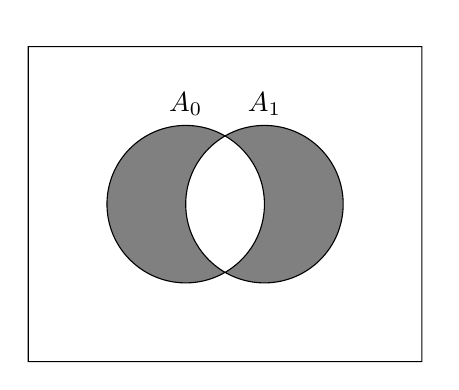
\begin{tikzpicture}[fill=gray]
	% left hand
	\scope
	\clip (-2,-2) rectangle (2,2)
	      (1,0) circle (1);
	\fill (0,0) circle (1);
	\endscope
	% right hand
	\scope
	\clip (-2,-2) rectangle (2,2)
	      (0,0) circle (1);
	\fill (1,0) circle (1);
	\endscope
	% outline
	\draw (0,0) circle (1) (0,1)  node [text=black,above] {$A_0$}
	      (1,0) circle (1) (1,1)  node [text=black,above] {$A_1$}
	      (-2,-2) rectangle (3,2) node [text=black,above] {};
	\end{tikzpicture}
\end{center}


\section{Random Variables}
A random variable $X$ is a function $X : U \rightarrow V$

\subsection{Example}
\begin{gather*}
X : \{ 0,1 \}^n \rightarrow \{ 0,1 \} \; ; \; X(y) = lsb(y) \in \{0,1\}
\end{gather*}

\noindent
For the uniform distribution on $U$:
\begin{gather*}
	Pr [X=0] = \frac{1}{2} \; , \; Pr [X=0] = \frac{1}{2}
\end{gather*}

\noindent
More generally, rand. var $X$ induces a distribution on $V$: 
\begin{gather*}
	Pr [X=v] := Pr \big[ X^{-1}(v) \big]
\end{gather*}

\section{The Uniform Random Variable}
Let $U$ be some set, e.g. $U = \{0,1\}^n$. We denote a \emph{\textbf{uniform random variable}} over $U$ as follows: 

\begin{gather*}
	\forall.a \in U : \; Pr [r = a] = \frac{1}{|U|}
\end{gather*}

\noindent
More formally, $r$ is the identity function: 

\begin{gather*}
	\forall.x \in U : \; r(x) = x
\end{gather*}

\todo{Finish Chapter 1!!!}

\chapter{Stream Ciphers}
\section{Symmetric Cipher}
\begin{definition}
A \textbf{cipher} defined over $( \mathscr{K,M,C} )$ is a pair of \textbf{polynomial time algorithms} $(E,D)$ such that:
\begin{gather}
	\begin{gathered}
		E : \mathscr{K} \times \mathscr{M} \rightarrow \mathscr{C} \\
		D : \mathscr{K} \times \mathscr{C} \rightarrow \mathscr{K} \\
		\textrm{s.t} \quad \forall m \in \mathscr{M},\; k \in \mathscr{K} : D(k, E(k, m)) = m
	\end{gathered}
\end{gather}
\end{definition}

\noindent
$\mathscr{K}$ is the key-space, $\mathscr{M}$ is the message-space and $\mathscr{C}$ is the ciphertext-space. The encryption algorithm $E$ is often randomized but the decryption algorithm $D$ is \emph{\textbf{always}} deterministic.

\section{One Time Pad\textsuperscript{\cite{1}}}

\begin{gather}
	\begin{gathered}
		\mathscr{M} = \mathscr{C} = \mathscr{K} = \{0,1\}^n			
	\end{gathered}	
\end{gather}

\noindent
In a one time pad the message, key and ciphertext spaces are the set of n-bit binary strings. A key $k \in \mathscr{K}$ is a \emph{random bit string} the length of the message, i.e. $|\mathscr{K}|=|\mathscr{M}|$.

\begin{gather}
	\begin{gathered}
		\exists. c \in \mathscr{C}, k \in \mathscr{K}, m \in \mathscr{M}: E(k, m) = k \oplus m = c
	\end{gathered}	
\end{gather}

\noindent
Given the encryption algorithm is an \emph{\textbf{xor}} of the key and message, we get that the ciphertext is also the same length as the key and the message, i.e. $|\mathscr{K}|=|\mathscr{M}|=|\mathscr{C}|$.

\begin{thebibliography}{9} 
	\bibitem{1} Gilbert Vernam patented the one time pad between 1918 and 1919, see \url{http://www.google.com/patents/US1310719}. (\todo{Expand on this a little, maybe...})
\end{thebibliography}
\end{document}